% !TEX root = ../main.tex

\chapter{Deep learning}
\label{ch:deep_learning}

\section{Introduction to deep learning}
Deep learning is currently one of the trendiest topics in machine learning, a subset of artificial intelligence. Machine learning refers to statistical models that allow computers to perform specific tasks without having been explicitly programmed to solve them. In fact, these models try to find structural patterns within data in order to understand new incoming situations and react in the best possible way accordingly. There exist various techniques in machine learning such as k-NN, SVM, k-means, decision trees, association rules, etc. What mainly differentiates deep learning from these algorithms is the concept of neural networks (see section  \ref{what_is_a_neural_network}), that are combined to form deep neural networks.\\
Neural networks are inspired from the biological neural networks of the brain. These systems try to learn how to solve a problem based on the data they receive as input. Many concrete applications make use of neural networks: autonomous vehicles, smarter translators, computer-aided diagnoses, personal assistants, art creation, robotics, etc. The presence of deep learning techniques in all mentioned use cases clearly attests that this technology is a real breakthrough. Furthermore, since this field has recently gained interest   (see section \ref{historical_background}), multiple researches are still ongoing, which suggests that many exciting new applications will certainly be discovered.

\subsection{Historical background}
\label{historical_background}
As described in figure \ref{history} from article \cite{14}, the theoretical foundations of deep learning appeared long before the invention of computers. From the first attempts to understand the human brain until today, a long way has been made to establish the basic components of modern neural networks. One could ask: why did deep learning take off recently if the theory has been around for a long time?\\
First part of the answer is about the computational power. Indeed, deep learning algorithms need a lot of data to work properly and this requires powerful CPU/GPU that either didn't exist or were only available to a minority of people. One other main reason concerns the lack of data. Since deep learning algorithms "learn" from data, if not data is available, no learning is possible. Consequently, the era of Big Data has enhanced the deep learning possibilities. These two points are summarised: "The increase in model size overtime, due to the availability of faster CPUs, the advent of general purpose GPUs, fasternetwork, connectivity and better software infrastructure for distributed computing, is one of the most important trends in the history of deep learning. This trend is generally expected to continue well into the future"\cite{15}.\\
Finally, before the year 2012, the abilities of neural networks had not been publicly proven. This changed with the ImageNet Large Scale Visual Recognition Challenge (a competition where researchers evaluate their algorithms on several visual recognition tasks). In fact, the deep convolutional neural network called "AlexNet" achieved 16\% of classification error rate, whereas the previous best scores were around 25\%. This victory marked the beginning of a new craze for these types of algorithms.



\begin{figure}[!h]
\centering
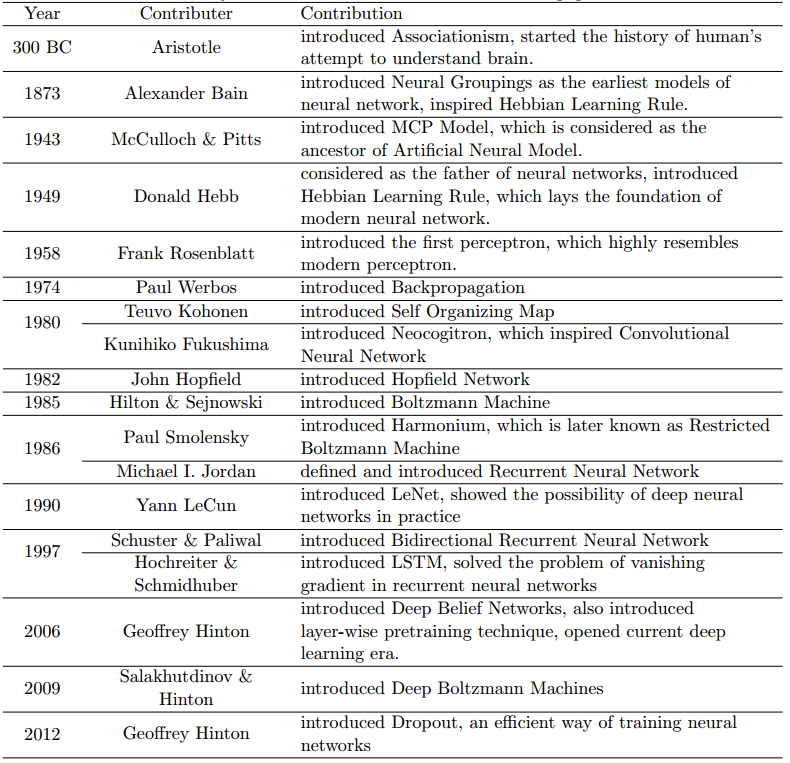
\includegraphics[width=1\textwidth, keepaspectratio=true]{./figures/history.png}
\caption{Milestones }
\label{history}
\end{figure}

 
\subsection{What is a neural network?}
\label{what_is_a_neural_network}

From a descriptive point of view, neural networks can simply be seen as a non linear applications that associate an input to an output with respect to certain parameters. The input can be images, sounds or whatever features that is numerical. The output of a neural network depends on the problem it tries to solve. In computer vision, the most common types of outputs  are classes (for classification problems) and pixel coordinates (for segmentation problems).\\
From a mathematical point of view, a neural network can be defined as a non linear function $f$ that associates to an input $x$ an output $y$ with respect to parameters $\theta$.
\begin{equation}
y = f(x,\theta)
\end{equation}
The parameters $\theta$ are estimated from the training samples.
%\begin{figure}[!h]
%\centering
%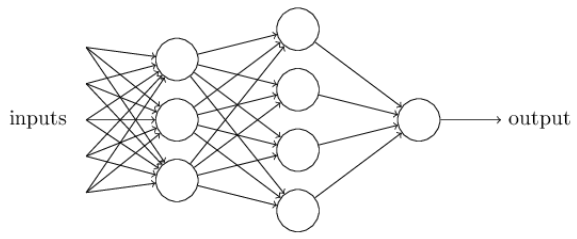
\includegraphics[width=1\textwidth, keepaspectratio=true]{./figures/neural_network.png}
%\caption{Neural Network example}
%\label{neural_network}
%\end{figure}

\subsection{Supervised learning and Unsupervised learning}
In machine learning, there mainly exists two different kinds of task. The first one is "supervised learning". It includes all learning algorithms, whose training samples contains labels in order to find the optimal mapping between the input and the output.  The second one is "unsupervised learning". In contrast to supervised algorithms, the latter use non labeled data and its main goal is to infer the natural structure  present in the data. Since the model presented in this work belongs to the "supervised learning" category, all notions explained below refer to this kind of algorithms.





\section{Neural networks basics}

\subsection{Notation}
In order to respect a consistent mathematical notation to describe neural networks, this work will use the notation of Andrew Y. Ng, one of the pioneers of deep learning, that can be found in \cite{16}.\\

\noindent \textbf{General comment}
\begin{itemize}
\item Superscript (i) will denote the $i^{th}$ training example.
\item Superscript [l] will denote the $l^{th}$ layer of the neural network.
\end{itemize}

\noindent \textbf{Sizes}
\begin{itemize}
\item $m$: number of examples in the dataset.
\item $n_{x}$: input size.
\item $n_{y}$: output size (or number of classes).
\item $n_{h}^{[l]}$: number of hidden units (i.e neurons) of the $l^{th}$ layer. 
\item $L$: number of layers in the network.
\end{itemize}

\noindent \textbf{Neural networks components}
\begin{itemize}
\item $X\in \R$ is the input matrix matrix of a neural network.
\item $x^{(i)} \in \R^{n_{x}}$ is the $i^{th}$ example (sample) represented as a column vector.
\item $Y \in \R^{n_{y} \times m}$ is the label matrix.
\item $y^{(i) \in \R^{n_{y}}}$ is the output label for the $i^{th}$ example.
\item $W^{[l]} \in \R$ \textsuperscript{\# of neurons in the next layer = j  x \# of neurons in the previous layer = k} is the weight matrix at layer $[l]$.
\item $b^{[l]} \in R$\textsuperscript{\# of units in next layer} is the bias vector in the $l^{th}$ layer.
\item $\hat{y} \in R^{n_{y}}$ is the predicted output vector. It can also be denoted $a^{[L]}$ where $L$ is the number of layers in the network.
\item $g^{[l]}(x)$ is the $l^{th}$ activation function.  
\item $z^{[l]} = W_{x}x^{(i)} + b^{[l]}$ denotes the weighted sum of the input given to the $l^{th}$ layer before passing through the activation function.\\
\end{itemize}

\noindent \textbf{Forward propagation equations}
\begin{itemize}
\item $a = g^{[l]}(W_{x}x^{(i)} + b^{[l]}) = g^{[l]}(z^{[l]})$ where $g^{[l]}$ denotes the $l^{th}$ layer activation function.
\item $a_{j}^{[l]} = g^{[l]} (\sum_{k} w_{jk}^{[l]}a_{k}^{[l-1]} + b_{j}^{[l]}) = g^{[l]} (z_{j}^{[l]}) $ is the general activation formula at $l^{th}$ layer.
\item $J(x, W, b, y) or J(\hat{y}, y)$ denote the cost function.
\end{itemize}

\subsection{Perceptrons}
\label{perceptron}
Perceptrons are the main components of neural networks. They were "developed in the 1950s and 1960s by the scientist Frank Rosenblatt, inspired by earlier work by Warren McCulloch and Walter Pitts"\cite{13}. Today, they are called "artificial neurons" or simply "neurons".\\
A perceptron $j$ is a function $f$ of the input $x=(x_{1}, ..., x_{n})$ weighted by a vector of weights $w_{}=(w_{1}, ..., w_{n})$, completed by a bias $b_{j}$ and associated to a non linear activation function $g$:
\begin{equation}
\label{perceptron_equation}
a_{j} = f_{j}(x) = g((\sum_{k=1}^{n} x_{k} * w_{k}) + b_{})
\end{equation}

Schematically, a perceptron can be represented as shown in figure \ref{perceptron_model}. Each input is multiplied with its corresponding weight and the sum of this result is then passed through a non linear function, called an "activation function". This activation function acts like a threshold that decides the proportion of the result that has to be given further. There exist multiple activation functions (see \ref{activation_functions}). It is extremely important to use a non linear functions instead of a linear function. Indeed, in a neural network the output of a perceptron is given as input to the others (see \ref{multilayer_perceptron}). Consequently, if only linear functions are used, linear outputs are given as inputs to other linear functions. Since the composition of two linear functions is itself a linear function, there would be no sense to assemble perceptrons to create neural networks of multiple layers.


\tikzset{basic/.style={draw,fill=white!20,text width=1em,text badly centered}}
\tikzset{input/.style={basic,circle}}
\tikzset{weights/.style={basic,rectangle}}
\tikzset{functions/.style={basic,circle,fill=white!10}}



\begin{figure}[!h]
\centering
	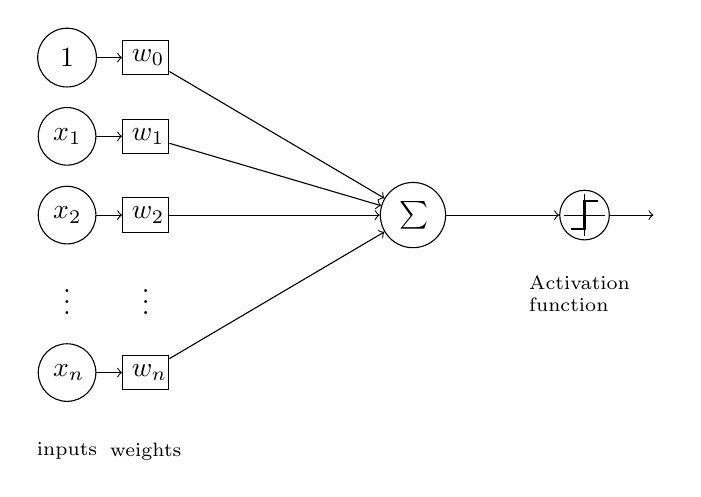
\begin{tikzpicture}
	
	\node[functions] (center) {};
        \node[below of=center,font=\scriptsize,text width=4em] {Activation function};
        \draw[thick] (0.5em,0.5em) -- (0,0.5em) -- (0,-0.5em) -- (-0.5em,-0.5em);
        \draw (0em,0.75em) -- (0em,-0.75em);
        \draw (0.75em,0em) -- (-0.75em,0em);
        \node[right of=center] (right) {};
            \path[draw,->] (center) -- (right);
        \node[functions,left=5em] (left) {$\sum$};
            \path[draw,->] (left) -- (center);
        \node[weights,left=15em] (2) {$w_2$} -- (2) node[input,left of=2] (l2) {$x_2$};
            \path[draw,->] (l2) -- (2);
            \path[draw,->] (2) -- (left);
        \node[below of=2] (dots) {$\vdots$} -- (dots) node[left of=dots] (ldots) {$\vdots$};
        \node[weights,below of=dots] (n) {$w_n$} -- (n) node[input,left of=n] (ln) {$x_n$};
            \path[draw,->] (ln) -- (n);
            \path[draw,->] (n) -- (left);
        \node[weights,above of=2] (1) {$w_1$} -- (1) node[input,left of=1] (l1) {$x_1$};
            \path[draw,->] (l1) -- (1);
            \path[draw,->] (1) -- (left);
        \node[weights,above of=1] (0) {$w_0$} -- (0) node[input,left of=0] (l0) {$1$};
            \path[draw,->] (l0) -- (0);
            \path[draw,->] (0) -- (left);
        \node[below of=ln,font=\scriptsize] {inputs};
        \node[below of=n,font=\scriptsize] {weights};
	
	\end{tikzpicture}
\caption{The perceptron model}
\label{perceptron_model}
\end{figure}

\subsection{Activation functions}
\label{activation_functions}
Once the computation of the weighted sum of all inputs for a specific neuron is done, the latter has to pass the sum through an activation function that will decide the proportion of the result to send further. Activation functions have to be non-linear in order to approximate extremely complex functions. In fact, neural networks are considered as universal approximators. Article \cite{17} claims that "multilayer feedforward networks are capable of approximating any measurable function to any desired degree of accuracy, in a very specific and satisfying sense."According to \cite{18} the most commonly used activation functions are:\\\\
 \noindent \textbf{Sigmoid function}\\
 The sigmoid function is defined as:
 \begin{equation}
  g(x) = \frac{1}{1+e^{-x}}
 \end{equation}
 Its derivative is:
 \begin{equation}
 g'(x) = g(x)(1-g(x))
 \end{equation}
 


\begin{figure}[h!]
  \begin{center}
    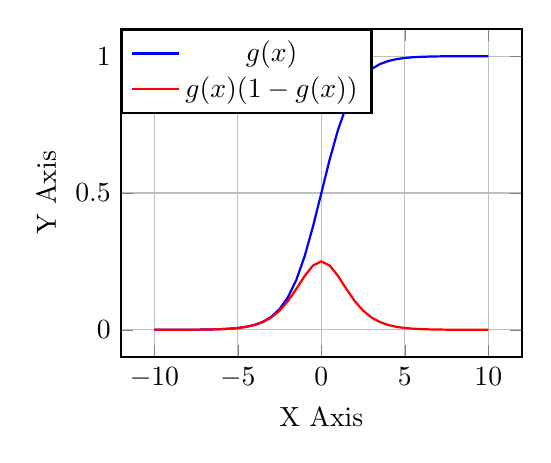
\begin{tikzpicture}
      \begin{axis}[
      	  width=0.55\linewidth, % Scale the plot to 0.7 \linewidth
          xlabel={$x$}, 
          ylabel={$y$},
          xlabel=X Axis, 
          ylabel=Y Axis,
          samples=41, 
          grid, 
          thick,
          domain=-10:10,
		legend style={at={(0,1)},anchor=north west}
        ]
        \addplot+[no marks] {1/(1+exp(-x))};
        \addlegendentry{$g(x)$}
        \addplot+[no marks] {(1/(1+exp(-x))) * (1-(1/(1+exp(-x))))};
        \addlegendentry{$g(x)(1-g(x))$}
      \end{axis}
    \end{tikzpicture}
    \caption{The sigmoid function and its derivative}
  \end{center}
\end{figure} 
 
 
 \noindent \textbf{Tanh function}\\
 \begin{equation}
 g(x) = tanh(x) = \frac{1-e^{-2x}}{1+e^{-2x}}
 \end{equation}
 Its derivative is:
 \begin{equation}
 g'(x) = tanh'(x) = 1-tanh^{2}(x)
 \end{equation}
 
  \begin{figure}[h!]
  \begin{center}
    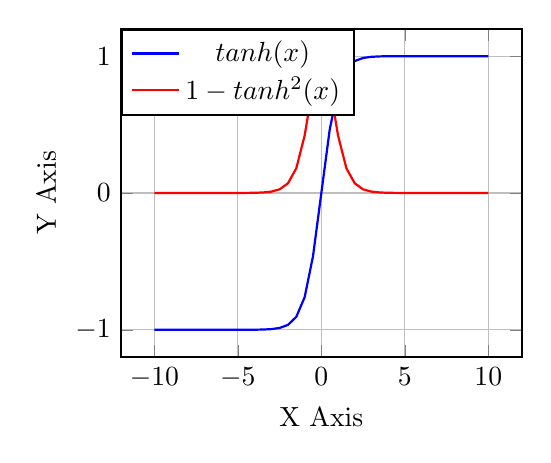
\begin{tikzpicture}
      \begin{axis}[
      	  width=0.55\linewidth, % Scale the plot to 0.7 \linewidth
          xlabel={$x$}, 
          ylabel={$y$},
          xlabel=X Axis, 
          ylabel=Y Axis,
          samples=41, 
          grid, 
          thick,
          domain=-10:10,
		legend style={at={(0,1)},anchor=north west}
        ]
        \addplot+[no marks] {(1-exp(-2*x))/(1+exp(-2*x))};
        \addlegendentry{$tanh(x)$}
        \addplot+[no marks] {1-((1-exp(-2*x))/(1+exp(-2*x)))^2};
        \addlegendentry{$1-tanh^{2}(x)$}
      \end{axis}
    \end{tikzpicture}
    \caption{The tanh function and its derivative}
  \end{center}
\end{figure} 
 
 \noindent \textbf{ReLU function}\\
 \begin{equation}
 g(x) = ReLU(x) = 
 \begin{cases}
    1 & \text{if } x\geq 0\\
    0              & \text{otherwise}
\end{cases}
 \end{equation}
 
 \begin{figure}[h!]
  \begin{center}
    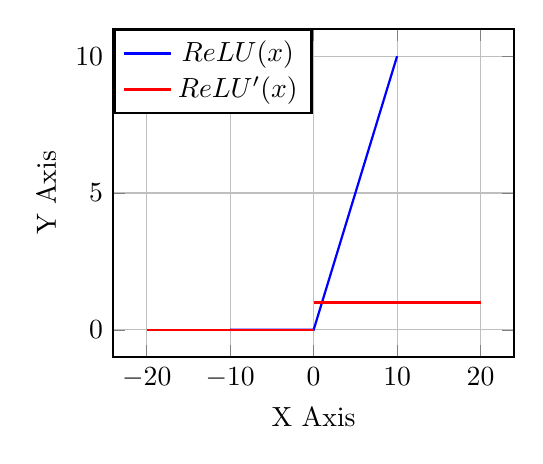
\begin{tikzpicture}[
    declare function={
    func(\x)= (\x<=0) * (0);
  }
  ]
      \begin{axis}[
      	  width=0.55\linewidth, % Scale the plot to 0.7 \linewidth
          xlabel={$x$}, 
          ylabel={$y$},
          xlabel=X Axis, 
          ylabel=Y Axis,
          samples=41, 
          grid, 
          thick,
          domain=-10:10,
		legend style={at={(0,1)},anchor=north west}
        ]
        \addplot+[no marks] {(x>=0)*x};
        \addlegendentry{$ReLU(x)$}
        \addplot[domain=-20:0,red] {0};
		\addplot[domain=0:20, red] {1};
        \addlegendentry{$ReLU'(x)$}
      \end{axis}
    \end{tikzpicture}
    \caption{The ReLU function and its derivative(not defined when x=0)}
  \end{center}
\end{figure} 
 
 
 
 
 \noindent \textbf{ELU function}\\
 \begin{equation}
 g(x) = 
 \begin{cases}
    x & \text{if } x\geq 0\\
    e^{x}-1 & \text{otherwise }
\end{cases}
 \end{equation}
 Its derivative is:
 \begin{equation}
g'(x) = 
 \begin{cases}
    1 & \text{if } x\geq 0\\
    e^{x} & \text{otherwise }
\end{cases}
 \end{equation}
 
 

  \begin{figure}[h!]
  \begin{center}
    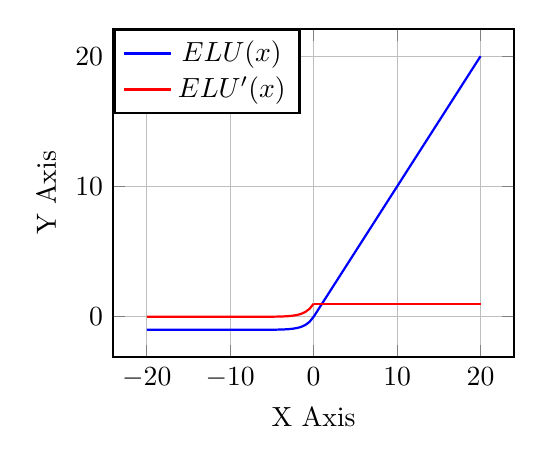
\begin{tikzpicture}[
    declare function={
    func(\x)= (\x>=0) * (x) +and (\x<0) * 4;
  }
    ]
      \begin{axis}[
      	  width=0.55\linewidth, % Scale the plot to 0.7 \linewidth
          xlabel={$x$}, 
          ylabel={$y$},
          xlabel=X Axis, 
          ylabel=Y Axis,
          samples=41, 
          grid, 
          thick,
          domain=-10:10,
		legend style={at={(0,1)},anchor=north west}
        ]
        \addplot[domain=0:20, blue] {x};
        \addlegendentry{$ELU(x)$}
        \addplot[domain=0:20,red] {1};
        \addlegendentry{$ELU'(x)$}
          
        \addplot[domain=-20:0,red] {exp(x)};
        \addplot[domain=-20:0,blue] {exp(x)-1};
        
      \end{axis}
    \end{tikzpicture}
    \caption{The ELU function and its derivative}
  \end{center}
\end{figure} 

\subsection{Multilayer perceptrons}
\label{multilayer_perceptron}
A multilayer perceptron is an artifical neural network type. Article \cite{23} defines the multilayer perceptrons as "feedforward networks with one or more layers of units between the
input and output layers. The output units represent a hyperplane in the space
of the input patterns."\\
A multilayer perceptrons is composed of $L$ layers each of them having $n^{l}_{h}$ perceptrons. The layers are organized in the following way:
\begin{itemize}
\item The input layer: it is the neural network entry point for the data. Generally, the data is provided to the network in the form of a matrix $X \in \R$ of size $(n_{x} \times batch\_size)$ with their corresponding labels $Y \in \R$ of size $(n_{y} \times batch\_size)$. The batch size defines the number of samples that will be given at the same time to the network and $n_{x}$ is their dimension. Moreover, $x^{(i)}$ is the $i^{th}$ sample represented as a column vector. The total number of training samples is given by $m$. Finally, $y^{(i)}$ is the output label for the $i^{th}$ example. For instance, under the assumption that the number of samples is 100 and that the batch size is 32, 4 batches in total will be given as input to the network.
\item The hidden layer(s): hidden layers stand for all layers that are between the input layer and the output layer. For each of them are associated weights and biases (W, b), respectively denoted by $W^{[l]} \in \R $ and $b^{[l]}$, where $W_{ij}^{l}$ correspond to the weights associated with the connection between perceptron $j$ in layer $l$ and perceptron $i$ in layer $l+1$. By analogy, $b_{i}^{[l]}$ is the bias associated with perceptron $i$ in layer $l+1$. The weights and the biases of the network are the parameters that have to be optimized in order to have the best mapping between the inputs and the output of the network (see section \ref{training_a_neural_network} ). Before training the neural network, the weights can be randomly initialized or initialized with more sophisticated methods such as "Xavier initialization" or "Kaiming initialization"(see section \ref{weight_initialization}).
\item The output layer: it is the last layer of the neural network. Its role is essential since it produces the prediction of the network for a given input. The prediction of a neural network is given by $\hat{y} \in R^{n_{y}}$ with $n_{y}$ beeing the number of different labels. In a classification task, whose goal is to assign to each input a specific class, the $\hat{y}$ could be the probability of belonging to each class. In that case, the \textit{softmax} activation function would be used.
\end{itemize}
The advantage of organizing the weights, biases and inputs in matrices is due to the ability of modern CPU/GPU to quickly perform linear algebra computations. This way of structuring the network component is called "vectorization" and avoids at most using loops in the code, which could considerably slow down the computations.
The figure \ref{multilayer_perceptrons_figure} globally illustrates the concept of a multilayer perceptrons. In this example, the total number of layers $L$ is equal to 3, the input size $n_{x}$ is equal to 4 and the number of units in in each layer is $n_{h}^{1}= 4$, $n_{h}^{2}=2$, $n_{h}^{3}=1$. The network has the weights  $W^{(1)} \in \R^{2x3}$, $W^{(2)} \in \R^{1x2}$  and the biases  $b^{[1]}=2$, $b^{[2]}=1$.


\begin{figure}[!h]
\centering
	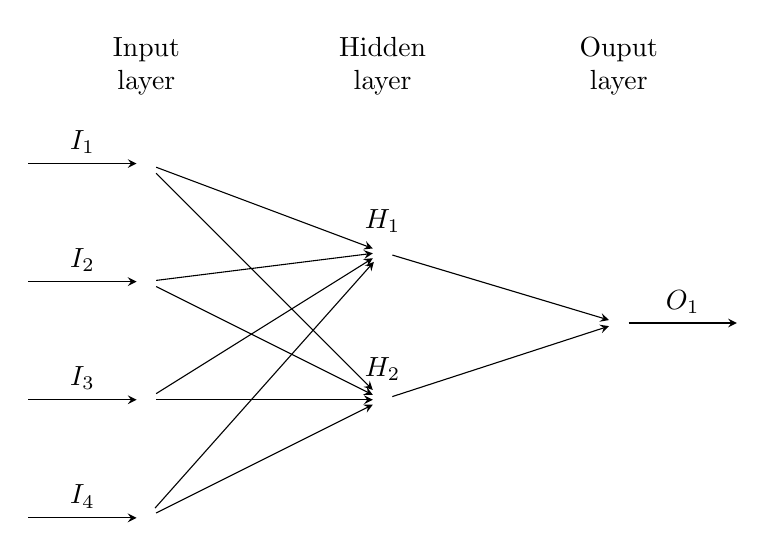
\begin{tikzpicture}[x=1.5cm, y=1.5cm, >=stealth]
	
	\foreach \m/\l [count=\y] in {1,2,3,4}
	  \node [every neuron/.try, neuron \m/.try] (input-\m) at (0,2.5-\y) {};
	
	\foreach \m [count=\y] in {1,2}
	  \node [every neuron/.try, neuron \m/.try ] (hidden-\m) at (2,2-\y*1.25) {};
	
	\foreach \m [count=\y] in {1}
	  \node [every neuron/.try, neuron \m/.try ] (output-\m) at (4,0.15) {};
	
	% input layer
	\foreach \l [count=\i] in {1,2,3,4}
	  \draw [<-] (input-\i) -- ++(-1,0)
	    node [above, midway] {$I_\l$};
	
	% hidden layer
	\foreach \l [count=\i] in {1,2}
	  \node [above] at (hidden-\i.north) {$H_\l$};
	
	% output neurons
	\foreach \l [count=\i] in {1}
	  \draw [->] (output-\i) -- ++(1,0)
	    node [above, midway] {$O_\l$};
	
	% input -> hidden
	\foreach \i in {1,...,4}
	  \foreach \j in {1,...,2}
	    \draw [->] (input-\i) -- (hidden-\j);
	
	% hidden -> output
	\foreach \i in {1,...,2}
	  \foreach \j in {1}
	    \draw [->] (hidden-\i) -- (output-\j);
	
	% labels above layers
	\foreach \l [count=\x from 0] in {Input, Hidden, Ouput}
	  \node [align=center, above] at (\x*2,2) {\l \\ layer};
	
	\end{tikzpicture}
\caption{Multilayer perceptrons}
\label{multilayer_perceptrons_figure}
\end{figure}

\section{Training a neural network}
\label{training_a_neural_network}
Training a neural network is composed of multiple steps. The first one is the "forward propagation step". It consists in giving to the untrained neural network examples that need to be classified (or segmented, depending on the task) and to transmit them through all layers of the network. Passing all batches as input to a network is called an "epoch". At the end of each batch the loss is computed using a "loss function". The latter is used to evaluate the predictions of the neural network in comparison to their ground-truth. Then, the weights and biases of the networks are updated during a process called "backpropagation" in order find the global minima of the loss function. This process is repeated for a defined number of epochs.



\subsection{Forward propagation}
The forward propagation is used to transmit the input through the entire neural network. Mathematically, the forward propagation for a given layer $l$ is given by two equations:
\begin{equation}
z^{[l]} = W_{x}^{[l]}x^{(i)} + b^{[l]}
\end{equation}
This first equation denotes the weighted sum of the input given to the $l^{th}$ layer before passing through the activation function $g$. The second equation describes the effect of the activation function:
\begin{equation}
a^{[l]} = g^{[l]}(z^{[l]})
\end{equation}
Since the output of the activation function is then given as input to all neurons of the next layer, the forward propagation step can be generally defined as:
\begin{equation}
a_{j}^{[l]} = g^{[l]} (\sum_{k} w_{jk}^{[l]}a_{k}^{[l-1]} + b_{j}^{[l]}) = g^{[l]} (z_{j}^{[l]}) 
\end{equation}
The figure \ref{forward_propagation} illustrates the computation of the forward propagation for the $l^{th}$ layer. The matrix of weight $W_{jk}^{l}$ correspond to the weights associated with the connection between perceptron $k$ in layer $l$ and perceptron $j$ in layer $l+1$. The latter is multiplied by the output of previous layer $a_{j}^{[l-1]}$, the biased $b^{[l]}$ is added and the entire result is given as input to the activation function.

\begin{figure}[!h]
\centering
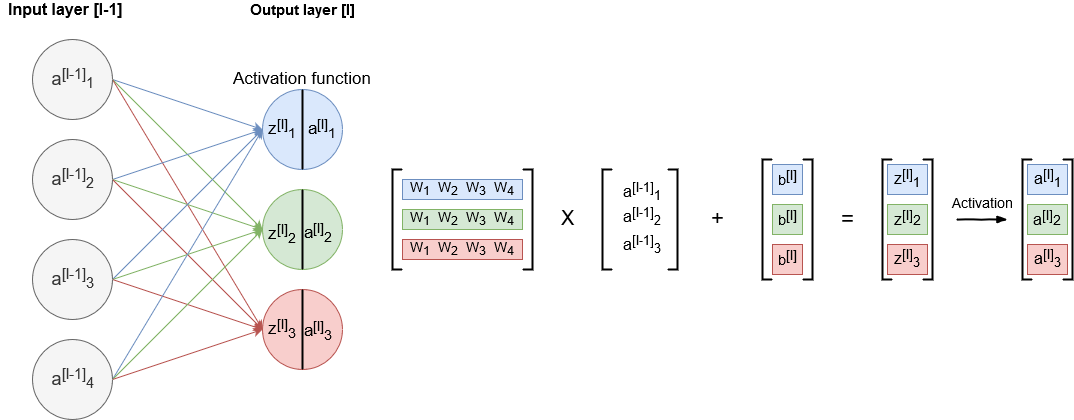
\includegraphics[width=1\textwidth, keepaspectratio=true]{./figures/forward_propagation.png}
\caption{Forward propagation }
\label{forward_propagation}
\end{figure}

\subsubsection{Loss computation}
"The loss function evaluates the error performed by the neural network when it tries
to estimate the data to be predicted"\cite{18}. It is therefore useful to measure the penalty for a single input. On the contrary, when the goal is to have a more general overview of the error on the entire batch or on the entire dataset, the cost function $J$ is used. The latter is given by $J(\hat{y}, y)$ where $\hat{y}$ is the prediction of the neural network and $y$ the real label. There exist multiple cost functions.\\
For a regression problem, a commonly used loss function is the mean square error:
\begin{equation}
J(\hat{y}, y) = \frac{1}{m}[\sum_{i=1}^{m} (\hat{y}^{(i)} - y^{(i)})^{2}]
\end{equation}
For classification problems, the cross entropy function is regularly used. We distinguish the binary classification where the number of classes $n_{y}$ = 2 and the multiclass classification where $n_{y}$ > 2. In binary classification, the cross entropy is:
\begin{equation}
J(\hat{y}, y) = -\frac{1}{m}\sum_{i=1}^{m} [y_{i}*log(\hat{y}_{i}) + (1-y_{i})*log(1-\hat{y_i})]
\end{equation}
In multiclass classification, the categorical crossentropy is:
\begin{equation}
J(\hat{y}, y) = - \sum_{i=1}^{n_{y}} \sum_{j=1}^{m} (y_{ij}*log(\hat{y}_{ij}))
\end{equation}

Since the cost function gives an estimation of the overall error of the network, the main objective of training a neural network is to update its weight in order to approach the minimum of the function. Therefore, deep learning problems can be considered as optimization problems. Solutions to these problems can be found using the gradient descent algorithm during backpropagation.
\subsection{Backpropagation}
Backpropagation relies on a technique called "gradient descent" to minimize the cost function $J(W, b)$. Globally, "the intuition behind the backpropagation algorithm is as follows. Given a training example $(x^{(i)}, y^{(i)})$, we will first run a forward pass to compute all the activations throughout the network, including the output value of the network. Then, for each node $i$ in layer $l$, we would like to compute an "error term" $\partial^{(l)}_{i}$ that measures how much that node was "responsible" for any errors in our output. For an output node, we can directly measure the difference between the network’s activation and the true target value, and use that to define $\partial^{(n_{l})}_{i}$(where layer $n_{l}$ is the output layer). How about hidden units? For those, we will compute $\delta^{(l)}_{i}$ based on a weighted average of the error terms of the nodes that uses $a^{(l)}_{i}$ as an input"\cite{24}.\\
In other words, after each forward pass through the entire network, backpropagation performs a backward pass with the goal of minimizing the cost function by adjusting model's parameters. The way parameters are updated is defined by the gradients of the cost function with respect to each parameter of the network. The gradient of the cost function $J(x_{1}, x_{2}, ..., x_{m})$ in point $x$ is given by:
\begin{equation}
\frac{\partial J}{\partial x} = [\frac{\partial J}{\partial x_{1}}, \frac{\partial J}{\partial x_{2}}, ..., \frac{\partial J}{\partial x_{1}}]
\end{equation}
The gradient shows how much all parameters that constitute x need to change to minimize the function. In neural networks, the parameters of the cost function are all weight matrices $W^{[l]}$ and biases $b^{[l]}$ The computation of all these gradients relies on the "chain rule". For weights parameters, the chain rule is:
\begin{equation}
\frac{\partial J}{\partial w_{jk}^{l}} = \frac{\partial J}{\partial z_{j}^{l}} * \frac{\partial z_{j}^{l}}{\partial w_{jk}^{l}}
\end{equation}
Similarly, the chain rules has to be applied to biases since they are also parameters of the cost function:
\begin{equation}
\frac{\partial J}{\partial b_{j}^{l}} = \frac{\partial J}{\partial z_{j}^{l}} * \frac{\partial z_{j}^{l}}{\partial b_{j}^{l}}
\end{equation}
Once the gradients of each parameters of the neural network are computed, they have to be updated. The weights update is described by the following equation:
\begin{equation}
W^{[l]} = W^{[l]} - \alpha * \frac{\partial J}{\partial W^{[l]}}
\end{equation}
The biases update corresponds to:
\begin{equation}
b^{[l]} = b^{[l]} - \alpha * \frac{\partial J}{\partial b^{[l]}}
\end{equation}
The hyperparameter $\alpha$ of these two equations is named "learning rate". It determines the gradient's influence at each epoch and has to be manually tuned.

\subsection{Metrics}
In classification tasks, four separate output labels can occur:
\begin{itemize}
\item True Positive (TP):  an output belongs to this class if the prediction that the latter \textbf{contains} a certain feature is \textbf{correct}.
\item True Negative (TN): an output belongs to this class if the prediction that the latter does \textbf{not contain} a certain feature is \textbf{correct}.
\item False Positive (FP): an output belongs to this class if the prediction that the latter \textbf{contains} a certain feature is \textbf{incorrect}.
\item False Negative (FN): an output belongs to this class if the prediction that the latter does \textbf{not contain} a certain feature is \textbf{incorrect}.
\end{itemize}
From these four categories, multiple metrics with their own specificities can be established \cite{25}:
\begin{itemize}
\item Accuracy: it is defined as the ratio of the correctly labeled subjects to the whole pool of subjects.
\begin{equation}
Accuracy = \frac{(TP+TN)}{TP+FP+FN+TN}
\end{equation}
Accuracy is a great measure in the case of symmetric data (i.e the number of FN $\approx$ FP and their cost is similar). When this condition is not fulfilled, accuracy can lead to bad models. For instance, let's define a binary classification model that always outputs class 0. If the data is composed of 99 samples from class 0 and 1 from class 1, the accuracy is equal to 99\% but the model is not smart. Consequently, this metric has to be used in addition to other metrics.

\item Precision: it is the ratio of the correctly positive labeled subjects by the model to all positive labeled subjects.
\begin{equation}
Precision = \frac{TP}{(TP + FP)}
\end{equation}
This metric is recommended when the confidence of the true positives predicted by the model is important. For instance, this happens in spam blockers where it is preferable to have a spam in mailbox rather than a regular mail in the spam box.

\item Recall (sensitivity):
\begin{equation}
Recall = \frac{TP}{(TP + FN)}
\end{equation}
This metric is recommended when the occurence of false negatives is intolerable and false positives are preferred. This makes perfect sense for disease detection models: labeling an healthy person as unhealthy is better than labeling an unhealthy person as healthy.

\item F1-score:
\begin{equation}
F1-score = \frac{2* recall * precision}{(recall + precision)}
\end{equation}
F1-score considers both precision and recall and is the highest if these two metrics are balanced. This metric is perfectly suitable when the cost of false positives and false negatives is not the same.

\item Specificity:
\begin{equation}
Specificity = \frac{TN}{(TN + FP)}
\end{equation}
This metric is recommended when the occurence of false positives is intolerable whereas true negatives are desired. For instance drug tests can not indicate false positives but they have to cover all true negatives.
\item AUC-ROC:
"The ROC curve is plotted with recall against the false positive rate (1-specificity) where recall is on y-axis and the false positive rate is on the x-axis. AUC - ROC curve is a performance measurement for classification problem at various thresholds settings. ROC is a probability curve and AUC represents degree or measure of separability. It tells how much model is capable of distinguishing between classes. Higher the AUC, better the model is at predicting 0s as 0s and 1s as 1s\cite{26}."

\end{itemize}




\subsection{Data}
In deep learning, data is essential. As seen previously, neural networks learn features from it. Therefore, data has to be handled carefully and in the right way. Usually, it is split into three different sets:
\begin{itemize}
\item The training set: this is the dataset that is used to train the neural network (the weights and biases).
\item The validation set: this the dataset that is used to evaluate a trained model.  Usually, the evaluation on the validation set is made every $x$ (a fixed number) epochs. The validation set needs to come from the same distribution as the training set but should contain exclusively unseen data. This last point is crucial since the validation set shows how well the neural network can generalize on unknown data. The validation set can also be used as indicator to decide when the training should be stopped in order to prevent "overfitting" (overfitting describes the behaviour of a model that too closely fits to the training set and don't generalize well). Indeed, if the validation loss continually increases for a certain number of epochs, going on with the training will increase the overfitting. This technique is called "early stopping".
\item The test set: this last dataset is used to establish the final evaluation of the model and also contains unseen data. 
\end{itemize}
Regarding the way these three sets are split, it mostly depends on the number of samples available. If the latter is big, the data is split into training and testing using the ratio 80/20. Then the remaining training samples are also split into training and validation using the ratio 80/20. On the contrary, if there are few data available, K-folds cross-validation is a good practice. This technique consists in splitting the entire dataset into k-folds. One fold is picked as test set and the others are considered as training sets. The model is trained on training folds and tested on the test set. Then, another test set is picked and the same process is repeated until all possible tests set are picked. At the end of the process, all results of all test sets are averaged, which provides a good estimation of the model performances. This technique is summarized on figure \ref{cross_validation}.

\begin{figure}[!h]
\centering
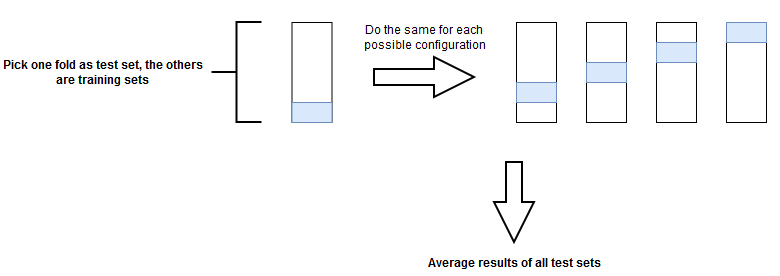
\includegraphics[width=1\textwidth, keepaspectratio=true]{./figures/cross_validation.png}
\caption{5-folds cross-validation }
\label{cross_validation}
\end{figure}


\subsection{Weight initialization}
\label{weight_initialization}
Before training a neural network, the weights have to be initialized in order to proceed to the first forward propagation. The initialization of the neural network weights is crucial since it will determine how quickly the network converges. The idea behind weight initialization is to generate an initialization that "prevents layer activation outputs from exploding or vanishing during the course of a forward pass through a deep neural network. If either occurs, loss gradients will either be too large or too small to flow backwards beneficially, and the network will take longer to converge, if it is even able to do so at all"\cite{27}.\\
The simplest and least efficient technique to initialize neural network weights is to randomly generate them. The major problem of this technique comes from the fact that some initializations can lead to extremely small or big values, which lead to value near 0 or 1 for most activation functions. Consequently, the slope of the gradient changes slowly and the learning takes a lot of time.\\
To prevent this effect when the tanh activation function is used, "Xavier initialization" multiplies the random initialization by the fraction:
\begin{equation}
\frac{\sqrt{6}}{\sqrt{n_{h}^{[l]}+n_{h}^{[l+1]}}}
\end{equation}
where $n_{h}^{[l]}$ is the number of incoming network connection to the layer and $n_{h}^{[l+1]}$ is the number of outgoing network connections from that layer.\\
For activation functions that are not symmetric about zero and don't have outputs inside [-1,1] such as ReLU or ELU, Kaiming initialization is an alternative. It consists in multiplying the random initialized matrix weight by:
\begin{equation}
\frac{\sqrt{2}}{\sqrt{n_{h}^{[l]}}}
\end{equation} 
where $n_{h}^{[l]}$ is the number of incoming connections coming into a given layer from the previous layer's output.

\subsection{Hyperparameters}
Hyperparameters denotes parameters that cannot be directly learned from the data. In deep learning,

lr, batch size, epochs, optimizer, learning rate decay, ...


From: https://stats.stackexchange.com/questions/153531/what-is-batch-size-in-neural-network
Batch size: 
Advantages of using a batch size < number of all samples:
It requires less memory. Since you train the network using fewer samples, the overall training procedure requires less memory. That's especially important if you are not able to fit the whole dataset in your machine's memory.

Typically networks train faster with mini-batches. That's because we update the weights after each propagation. In our example we've propagated 11 batches (10 of them had 100 samples and 1 had 50 samples) and after each of them we've updated our network's parameters. If we used all samples during propagation we would make only 1 update for the network's parameter


The smaller the batch the less accurate the estimate of the gradient will be. In the figure below, you can see that the direction of the mini-batch gradient (green color) fluctuates much more in comparison to the direction of the full batch gradient (blue color).


\section{Deep learning models}
xxx

\subsubsection{Convolutional Neural Networks}


\subsubsection{Recurrent Neural Networks}




\section{Transfer learning}




\section{Deep learning frameworks}